%%%%%%%%%%%%%%%%%%%%%%%%%%%%%%%%%%%%%%%%%%%%%%%%%%%%%%%%%%%%%%%
%
% Welcome to Overleaf --- just edit your LaTeX on the left,
% and we'll compile it for you on the right. If you open the
% 'Share' menu, you can invite other users to edit at the same
% time. See www.overleaf.com/learn for more info. Enjoy!
%
%%%%%%%%%%%%%%%%%%%%%%%%%%%%%%%%%%%%%%%%%%%%%%%%%%%%%%%%%%%%%%%


% Inbuilt themes in beamer
\documentclass{beamer}

% Theme choice:
\usetheme{CambridgeUS}

% Title page details: 
\title{Assignment 9} 
\author{Jarpula Bhanu Prasad - AI21BTECH11015}
\date{\today}
\logo{\large \LaTeX{}}

\usepackage{hyperref}
\usepackage{mathtools}
\usepackage{amssymb}
\usepackage{amsmath}


\begin{document}

% Title page frame
\begin{frame}
    \titlepage 
\end{frame}

% Remove logo from the next slides
\logo{}


% Outline frame
\begin{frame}{Papoulis chap 5 Ex 5.1}
TABLE OF CONTENTS
    \tableofcontents
\end{frame}


% Lists frame
\section{Question}
\begin{frame}{Problem}
Q)The distribution of $x^2$. 
\end{frame}

\section{Solution}
\begin{frame}{Solution}
    Let $y = x^2$ \\
    \begin{itemize}
        \item If $ y \ge 0 $, then $x^2 \le y$ for $-\sqrt{y} \le x \le \sqrt{y}$ (see fig\eqref{fig1}) .
        Hence \\ $F_y(y)=P(-\sqrt{y} \le x \le \sqrt{y})=F_x(\sqrt{y})-F_x({-}\sqrt{y})$  , $y>0$ \\ 
        
        \item  If $y<0$, then there are no values of $x$ such that $x^2 < y $.Hence \\
        $F_y(y)=P(\phi)=0$ ,$y<0$ \\

        \item By direct differentiation of $F_y(y)$, we get \\
        \begin{align}
            f_y(y) = 
            \begin{cases}
            \frac{f_x(\sqrt{y})+f_x({-}\sqrt{y})}{2 \sqrt[]{y}} & y>0 \\
            0 & \text{otherwise} 
            \end{cases}
            \label{1}
            \end{align}
        
    \end{itemize}

\end{frame}

\begin{frame}
    \begin{itemize}
        \item If $f_x(x)$ represents an even function, then eqn\eqref{1} reduces to 
        \begin{align} \label{2}
            f_y(y)= \frac{f_x(\sqrt{y})U(y)}{\sqrt{y}}
        \end{align}

        \item In particular if $x \thicksim N(0,1)$, so that 
        \begin{align} \label{3}
            f_x(x)=\frac{e^\frac{-x^2}{2}}{\sqrt{2\pi}}
        \end{align}
        and substituting this into eqn\eqref{2}, we obtain the p.d.f of $y = x^2 $ to be 
        \begin{align} \label{4}
            f_y(y)=\frac{e^\frac{-y}{2} U(y)}{\sqrt{2\pi y}}
        \end{align}
    \end{itemize}
\end{frame}

\begin{frame}
    On comparing this with $\textbf{CHI-SQUARE DISTRIBUTION}$,\\ we notice that eqn$\eqref{4}$ represent a chi-square random varaible with n=1, since $\varGamma(\frac{1}{2}) =  \sqrt{\pi}$. Thus, if $x$ is a Guassian random varaible with $\mu$ = 0, then $y=x^2$ represents a chi-square random varaible with one degree of freedom.
\end{frame}

\section{Graph}
\begin{frame}{$y = x^2$}
    \begin{figure}[!ht]
		\centering
		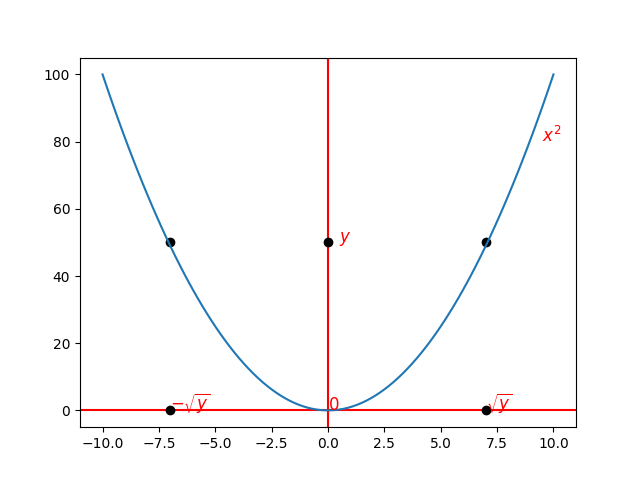
\includegraphics[width=\textwidth,height=5.5cm,keepaspectratio]{Figure_1}
		\caption{$y = x^2$}
		\label{fig1}
	\end{figure}
\end{frame}

% % Blocks frame
\section{Codes}
\begin{frame}{CODES}
    \begin{block}{Python}
         Download python code from - \href{https://github.com/jarpula-Bhanu/Assignment_9/blob/main/code/graph.py}{Python}
    \end{block}

 \begin{block}{Beamer}
         Download Beamer code from - \href{}{Beamer}
    \end{block}
\end{frame} 

\end{document}